\section{Phase 3: Translating the CFG to an AST}
\label{sec:cfgtoast}
The main purpose of this phase is to take the control flow given in the structure of the control flow graph (CFG) and translate it into a tree form consisting of nodes representing common programming constructs, e.g., jump statements. Furthermore, read and write expressions contained in the CFG are parsed and translated into subtrees in order to make the there structure explicit in the produced tree.

\subsection{Performing the Translation}
The tree this phase produces is an abstract syntax tree (AST) for a simple language that contains common program constructs, e.g., jump statements, read and write statements and conditional statements. The AST contains a node for each program construct. The root node is a \emph{program node} that contains a number of \emph{processes} and \emph{global variables}. A process has a number of \emph{blocks}. This is the basic structure of the AST and to explain the translation we look at how the CFG for the producer-consumer system is translated into an AST. Fig.~\ref{fig:producerast} shows a subtree of the AST where only the nodes from the \code{produce data} block of the \code{producer} process is shown.

\begin{figure}
\centering
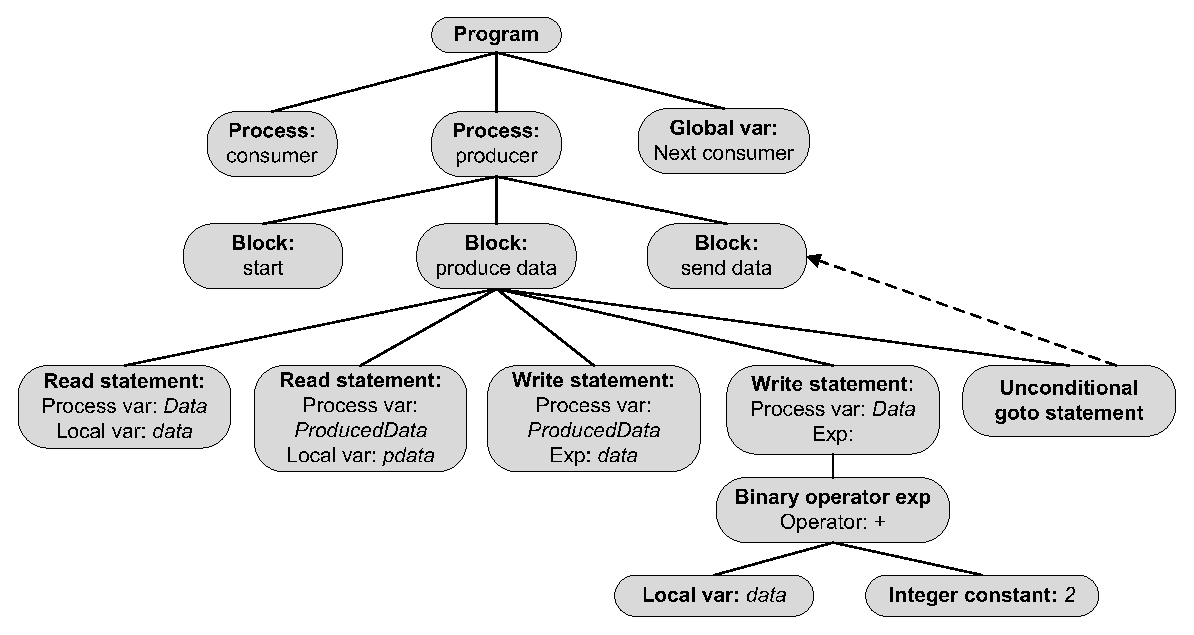
\includegraphics[width=\textwidth]{translation/cfg_to_ast/graphics/producerast.eps}
\caption{The AST for the "produce data" part of the producer}
\label{fig:producerast}
\end{figure}

When building the AST a process is created for each CFG process. As Fig.~\ref{fig:producerast} shows the program contains two processes, namely the \code{producer} and the \code{consumer}. The program node also contains the global variable \code{NextConsumer}. In the CFG each process contains a number of variables. These variables are translated into process variables local to each process. A process variable contains an initial expression for each instance of the process. Each initial expression is parsed and if not recognised an unknown expression is inserted. An AST process also has a number of AST blocks which are created from the basic blocks of the CFG. The \code{producer} process contains three blocks: \code{produce data}, \code{send data}, and \code{start}. Below, we explain how the block \code{produce data} is created.

\paragraph*{Read statements.} The first two child nodes in the \code{produce data} block are \emph{read statements}. These are translated from the two readings in the CFG of the process variables \code{Data} and \code{ProduceData}, respectively. A read statement contains both a \emph{local variable} and a \emph{process variable}. A local variable is a variable that is local to the block, and a process variable is local to the process. The value of a process variable is read into a local variable, e.g., the first read statement reads the value of the process variable \code{Data} into the local variable \code{data}.

\paragraph*{Write statements.} The next two nodes of the block are \emph{write statements} which write values to process variables. These are translated from the two writings in CFG to the process variables \code{ProduceData} and \code{Data}, respectively. Write statements contain an expression which becomes the new value of the process variable. The expression can, e.g., be the value of a local variable or an arithmetic expression.

The first write statement writes the value of the local variable \code{data} to the process variable \code{ProducedData}. The second write statement writes a value the process variable \code{Data}. This value is a binary operator expression which on the left hand side has the value of the local variable \code{data} and on the right hand side the integer constant \code{2}. This expression shows an example of how the structure of expressions are represented in the AST.

\paragraph*{Goto statements.} The rightmost node in the \code{produce data} block is an \emph{unconditional goto statement} which is a jump statement without a condition. It has a pointer to the block it jumps to which in this case is the \code{send data} block. The jump statements are translated from edges between basic blocks in the CFG. An AST has two types of goto statements, namely a unconditional without a condition, and a conditional which has a condition attached to it. The condition is a boolean expression specifying whether the jump should be made or not. Common for both types is that they have a pointer to an AST block which is the target of the goto statement.

\begin{figure}[b!]
\centering
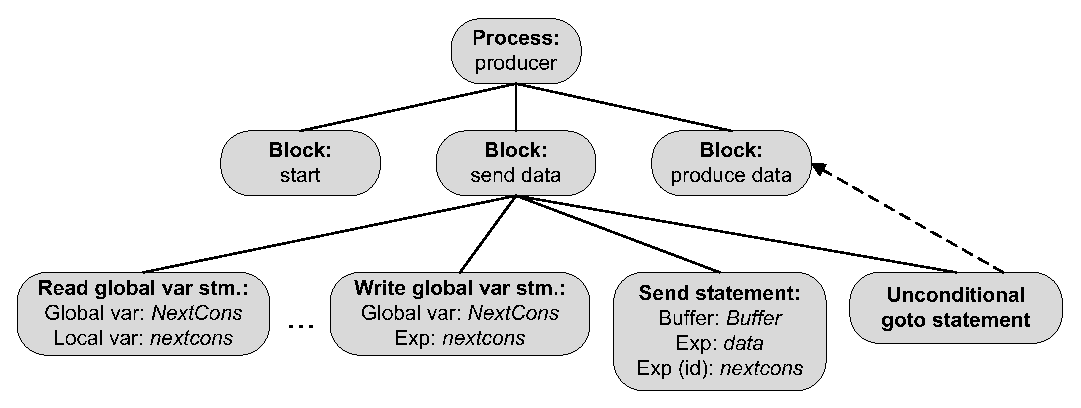
\includegraphics[scale=0.7]{translation/cfg_to_ast/graphics/producersendast.eps}
\caption{The AST for the "send data" part of the producer}
\label{fig:producersendast}
\end{figure}

\paragraph*{Read and write to and from global variables.}
Fig.~\ref{fig:producersendast} shows the "send data" part of the \code{producer} process. The three dots between the two first nodes indicates that we have left out a read and a write statement which reads the value of the process variable \code{ProducedData} into the local variable \code{data} and writes the same value back to \code{ProducedData} leaving it unchanged.

The first node in the \code{send data} block is a \emph{global variable read statement} which reads the value of the global variable \code{NextCons} into the local variable \code{nextcons}. This is very similar to a read statement from a process variable. The read statements of global variables are translated from the readings of global variables in the CFG.

The \emph{global variable write statements} are translated from writings of global variables from the CFG and are also very similar to writings to process variables. The second node in Fig.~\ref{fig:producersendast} writes the value of the local variable \code{data} to the global variable \code{NextCons}.

\paragraph*{Send statements.} The third node in the \code{send data} block is a \emph{send statement}. A send statement contains a pointer to the buffer that is to receive the message, and an expression that specifies the process identifier of the receiving process. With this information, a process is able to send a message to a specific buffer for a specific process. A send statement also contains an expression which specifies the value which is sent.

Send statements are translated from the send statements in the CFG. In Fig.~\ref{fig:producersendast} the send statement is to send the value of the local variable \code{data}, which was read from the process variable \code{ProducedData}. This value should be send to the buffer \code{Buffer} for the process which is identified by the value of \code{nextcons}, that was read from global variable \code{NextCons}.

\paragraph*{Receive statements.} Messages are received using a \emph{receive statement}. A receive statement has a pointer to a buffer where the incoming messages are stored and where the process can read the messages from. It also contains a local variable into which a message from the buffer is read. The receive statements are translated from the receive statements in the CFG. An example of the use of a receive statement is found in the \code{consumer} process when it receives the produced data from a \code{producer} process.

\subsection{The Structure of the AST}
% Forklar EBNF

\begin{figure}[b!]
\footnotesize
\begin{verbatim}
<Program>                    ::= *<Process> *<GlobalVariableDeclaration>
<GlobalVariableDeclaration>  ::= <Name> <InitialExpression>
<Process>                    ::= <Name> *<Block> <EntryBlock> 
                                        *<ProcessVariableDeclaration>
<Name>                       ::= string
<ProcessVariableDeclaration> ::= <Name> <InitialExpression>
<InitialExpression>          ::= <Expression>
<Block>                      ::= <Name> <Statements>
<EntryBlock>                 ::= <Block>
<Statements>                 ::= *<Statement> |
                                 <Statements> <UnconditionalGotoStatement>
<Statement>                  ::= <LocalVariableDeclaration> |
                                 <ReadStatement> | <ReceiveStatement> |
                                 <GlobalVariableReadStatement> |
                                 <WriteStatement> | <SendStatement> |
                                 <GlobalVariableWriteStatement> |
                                 <ConditionalGotoStatement>
...
<Expression>                 ::= <BinaryOperatorExpression> |
                                 <LocalVariableExpression> |
                                 <GlobalVariableExpression> |
                                 <ProcessVariableExpression> |
                                 <UnknownExpression> |
                                 <IntegerConstantExpression> |
                                 <StringExpression> | <Undefined>
...
\end{verbatim}
\normalsize
\caption{The EBNF for the abstract syntax tree}
\label{fig:ASTEBNF}
\end{figure}


In order to explain the structure of the AST more precisely we describe it using the Extended Backus-Naur Form (EBNF) \cite{EBNF}. Part of it is shown in Fig.~\ref{fig:ASTEBNF} and the full version can be found in appendix \ref{app:astebnffull}. The first definition is a \code{Program} which consists of zero or more processes and zero or more global variable declarations. A \code{GlobalVariableDeclaration} is a declaration of a variable that can be accessed by every running process in the program, i.e., a variable which is shared between processes. The \code{GlobalVariableDeclaration} consists of a name, which is a string, and an initial expression which is used to initialise the global variable.

A \code{Process} has a name which is simply a string. It has zero or more \code{Block}s which is a named block of statements. Furthermore, a \code{Process} has one or more \code{ProcessVariableDeclaration}s which is declarations of variables that can be accessed anywhere within the process. Finally, a \code{Process} has a \code{StartBlock} which is the first block of statements to be executed in the process.

Taking a closer look at the \code{Statement} and \code{Statements} constructions we see that they contain both a \code{ConditionalGotoStatement} and an \code{Unconditional}-\code{GotoStatement} which represents goto statements with or without an attached condition, respectively. The construction is made in such a way that if an \code{UnconditionalGotoStatement} appears there cannot appear other types of statements afterward. This is done to avoid unreachable statements.

The last construction in the EBNF is \code{Expression} which consists of all the types of expressions in the AST. We have chosen only to support a small set of expressions. E.g., we have chosen \emph{Binary Operator Expressions} to illustrate how expressions can be parsed from CPN ML into a tree structure fitting the AST. Other expressions are simply wrapped in an \code{UnknownExpression} which contains the expression as the original string. The type \code{Undefined} is used when, e.g., a variable has no initial value.
